% 
% ---------------------------------------------------------------
% Copyright (C) 2012-2018 Gang Li
% ---------------------------------------------------------------
%
% This work is the default powerdot-tuliplab style test file and may be
% distributed and/or modified under the conditions of the LaTeX Project Public
% License, either version 1.3 of this license or (at your option) any later
% version. The latest version of this license is in
% http://www.latex-project.org/lppl.txt and version 1.3 or later is part of all
% distributions of LaTeX version 2003/12/01 or later.
%
% This work has the LPPL maintenance status "maintained".
%
% This Current Maintainer of this work is Gang Li.
%
%

\documentclass[
 size=12pt,
 paper=smartboard, %a4paper, smartboard, screen
 mode=present, %present, handout, print
 display=slides, % slidesnotes, notes, slides
% nohandoutpagebreaks,
% pauseslide,
style=tuliplab,
% nopagebreaks,clock
% hlentries=true,
% hlsections = true,
pauseslide,
fleqn,leqno]{powerdot}

\hypersetup{pdfpagemode=FullScreen}
% \usepackage[toc,highlight,blackslide,slidesonly,sounds,HA]{HA-prosper}

\usepackage{amssymb}
\usepackage{amsmath} 
\usepackage{rotating}
\usepackage{graphicx}
\usepackage{boxedminipage}
\usepackage{media9}
\usepackage{rotate}
\usepackage{calc}
\usepackage[absolute]{textpos}
\usepackage{psfrag,overpic}
\usepackage{fouriernc}
\usepackage{pstricks,pst-node,pst-text,pst-3d,pst-grad}
\usepackage{moreverb,epsfig,color,subfigure}
\usepackage{color}
\usepackage{pstricks}
\usepackage{pstricks-add}
\usepackage{pst-text}
\usepackage{pst-node, pst-tree}
\usepackage{booktabs}
\usepackage{etex}
\usepackage{breqn}
\usepackage{multirow}
\usepackage{gitinfo2}


\usepackage{listings}
\lstset{frameround=fttt, 
frame=trBL, 
stringstyle=\ttfamily,
backgroundcolor=\color{yellow!20},
basicstyle=\footnotesize\ttfamily}
\lstnewenvironment{code}{
\lstset{frame=single,escapeinside=`',
backgroundcolor=\color{yellow!20},
basicstyle=\footnotesize\ttfamily}
}{}


\usepackage{fouriernc}
\usepackage{hyperref}

%%%%%%%%%%%%%%%%%%%%%%%%%%%%%%%%%%%%%%%%%%%%%%%%%%%%%%%%%%%%%%%%%%%%%%%%
% title
% TODO: Customize to your Own Title, Name, Address
%
\title{Digit Recognizer}
\author{
GengWang Li
\\
Flip00 
% \href{mailto:gangli@acm.org}{gangli@acm.org}
% \and % more authors
}
\date{\gitCommitterDate}


% Customize the setting of slides
\pdsetup{
% theslide=\arabic{slide}~/~\pageref*{lastslide},
% theslide=\arabic{slide},
rf=\href{http://www.tulip.org.au}{
Last Changed by: \textsc{\gitCommitterName}\ \gitVtagn-\gitAbbrevHash\ (\gitAuthorDate)
},
cf=\hyperlink{blankslide}{Flip00 Final Presentatin},
trans=Fade,
list={labelsep=1em,leftmargin=*,itemsep=0pt,topsep=5pt,parsep=0pt},
% counters={theorem,lemma},
% randomdots,dmaxdots=80
}


\begin{document}

\maketitle 

\begin{slide}[toc=,bm=]{Overview}
\tableofcontents[content=sections]
\end{slide}


\section{Introduction}

\begin{slide}[toc=,bm=]{Overview of the Introduction}
\tableofcontents[content=currentsection,type=1]
\end{slide}

\begin{slide}{Description of Competition}
  \begin{itemize}
    \item Competition \pause
    \begin{itemize}
      \item MNIST ("Modified National Institute of Standards and Technology") is the 
      de facto “hello world” dataset of computer vision.
    \end{itemize}
    \item Goal \pause
    \begin{itemize}
      \item goal is to correctly identify digits from a dataset of tens of thousands of handwritten images  
    \end{itemize}    
  \end{itemize}
\end{slide}

\begin{slide}{Dataset}
  \begin{itemize}
    \item Files\pause
      \begin{itemize}
        \item train.csv (contains 42000 items)
        \item test.csv (contains 28000 items)
        \item sample_submission.csv
      \end{itemize}
  \end{itemize}
  \pause
  \begin{figure}[h]
    \begin{minipage}[t]{0.4\linewidth}
    \centering
    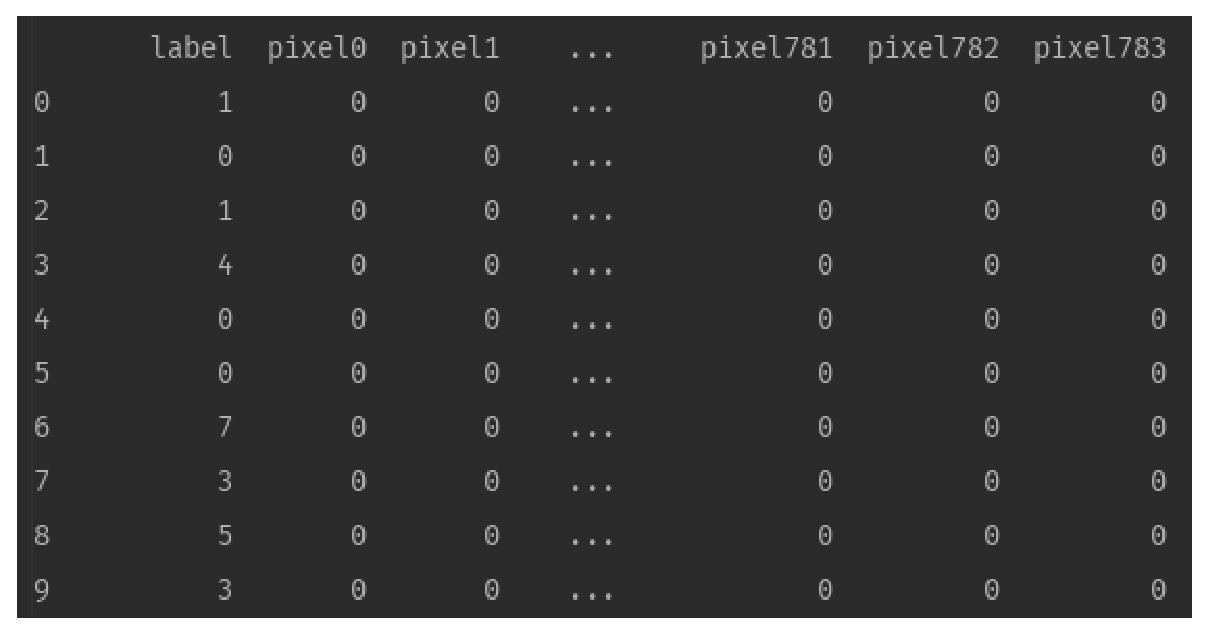
\includegraphics[width=1.2\textwidth]{figures/data-train.eps}
    \caption{train dataset}
    \label{fig:train-dataset}
    \end{minipage} 
    \hfill
    \begin{minipage}[t]{0.4\linewidth}
    \centering
    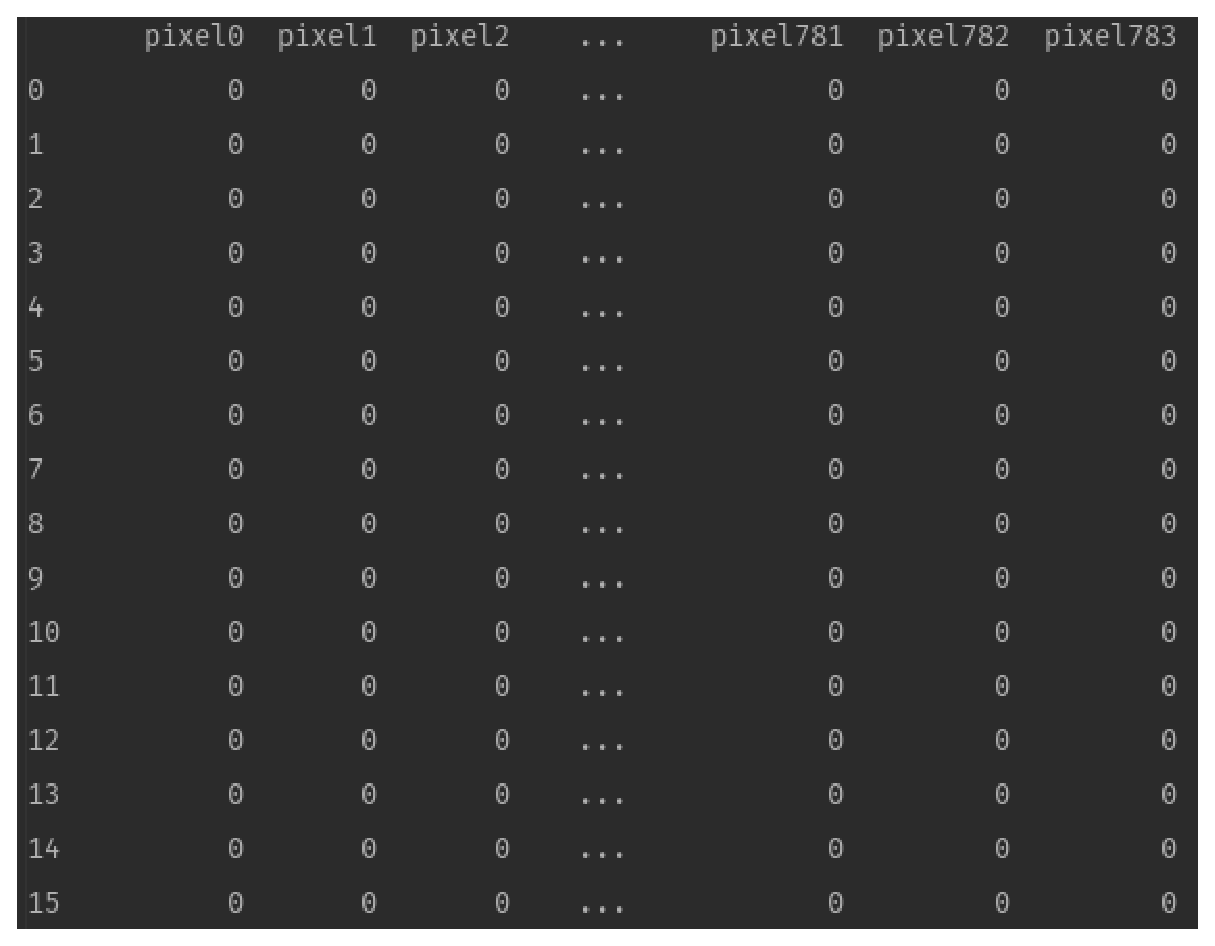
\includegraphics[width=1.2\textwidth]{figures/data-test.eps}
    \caption{test dataset}
    \label{fig:test-dataset}
    \end{minipage}
  \end{figure}
\end{slide}

\begin{slide}{Preview}
  \begin{itemize}
    \item Distribution of average pixels on different labels
  \end{itemize}
  \pause
  \begin{figure}[h]
    \centering
    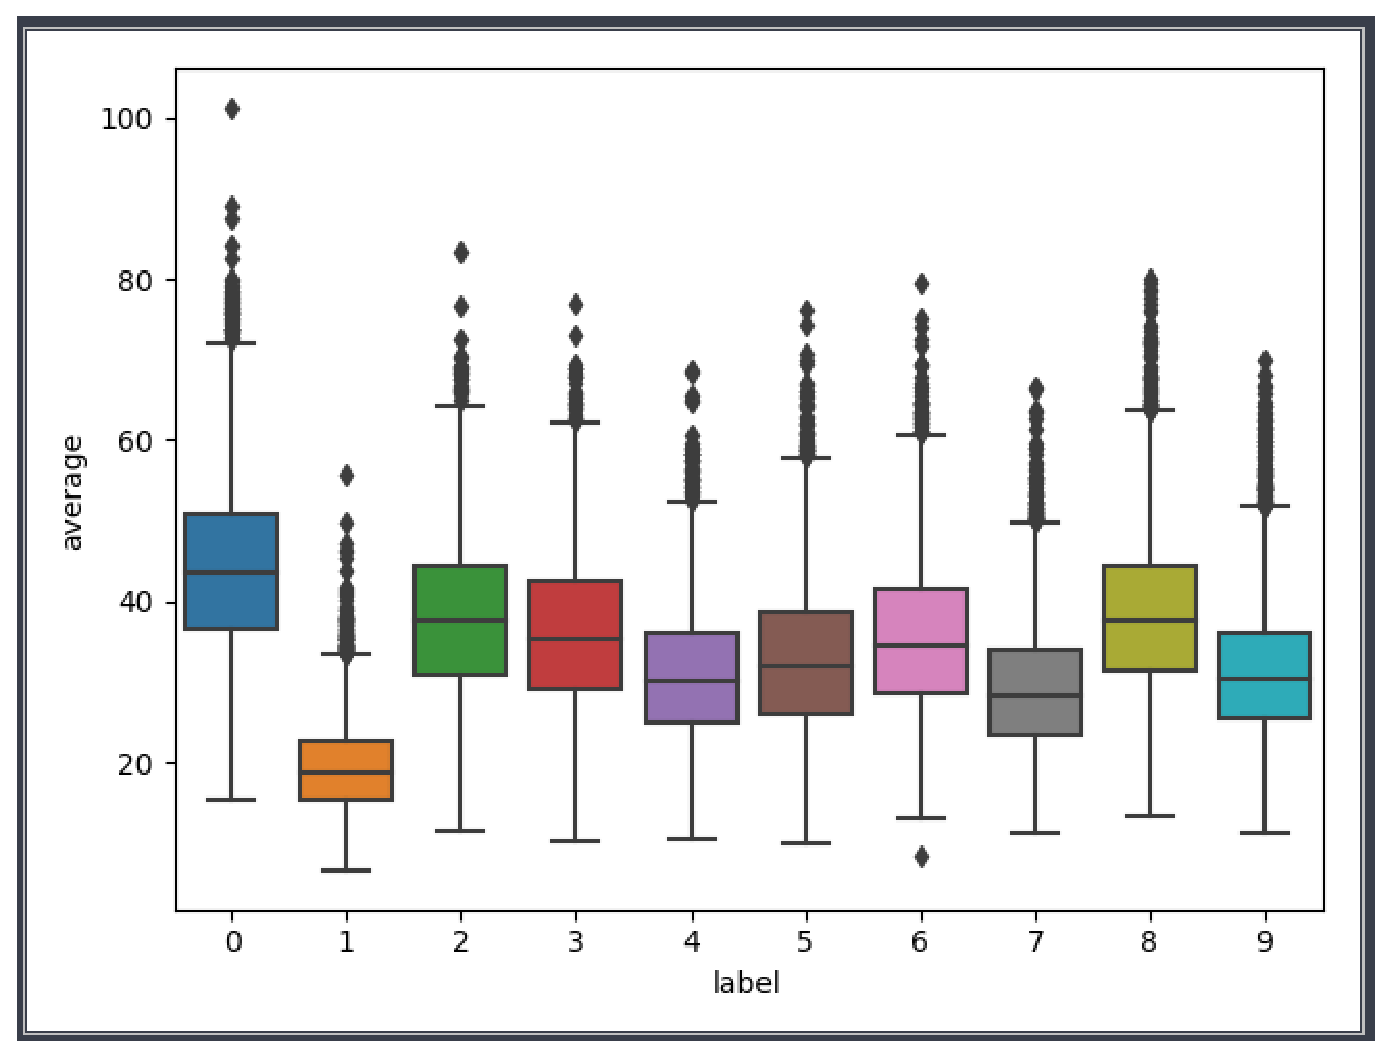
\includegraphics[width=0.5\linewidth]{figures/distribution-avg-pixels.eps}
    \caption{distribution of average pixels }
    \label{fig:distribution-avg-pixels}
  \end{figure}
\end{slide}


\section{Data Preprocess}

\begin{slide}{Data Visualization}
  \begin{itemize}
    \item Convert csv file into labeled pictures \pause
    \begin{figure}[h]
      \begin{minipage}[t]{0.4\linewidth}
        \centering
        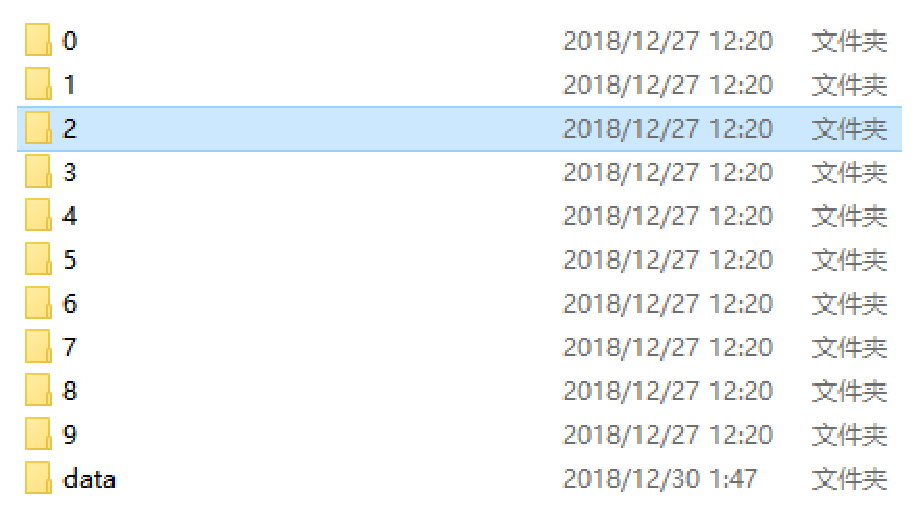
\includegraphics[width=1.2\textwidth]{figures/pic-categories.eps}
        \caption{categories of pictures}
        \label{fig:categories-picture}
      \end{minipage}
      \hfill
      \begin{minipage}[t]{0.4\linewidth}
        \centering
        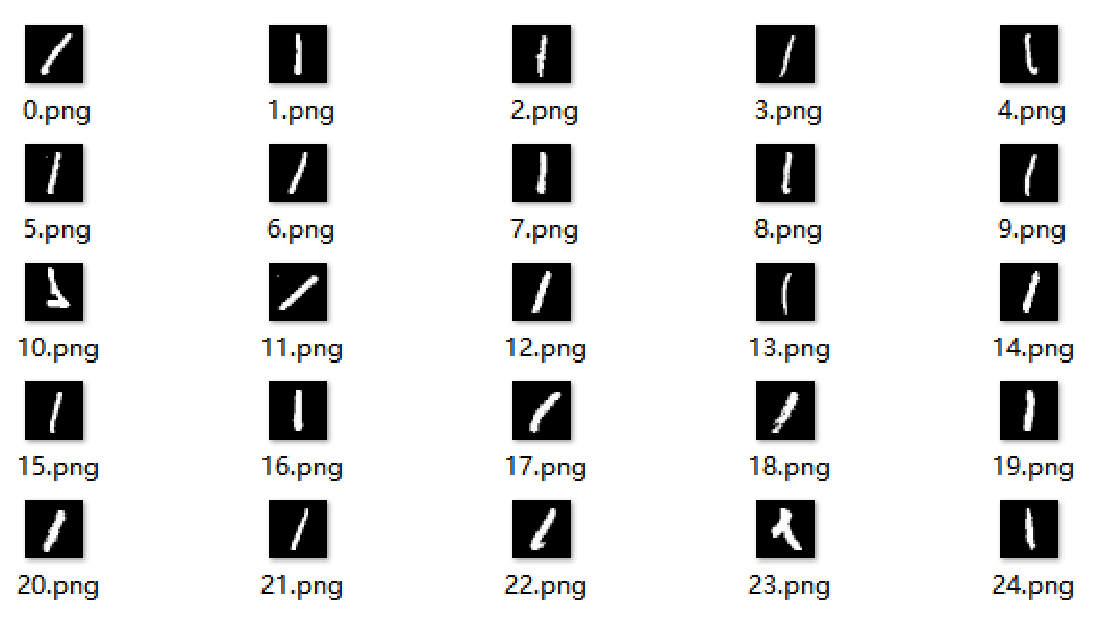
\includegraphics[width=1.2\textwidth]{figures/pic-label1.eps}
        \caption{pictures labeled as 1}
        \label{fig:pic-label1}
      \end{minipage} 
    \end{figure}
  \end{itemize}
\end{slide}

\begin{slide}{Normalization}
  \begin{itemize}
  \item All the 784 attributes of one example are gray values of pixel \pause
  \item Standard Normalization may be a bad idea \pause

  $$
  z = \frac{X-\mu}{\delta}
  $$
  \pause
  \begin{figure}[h]
    \centering
    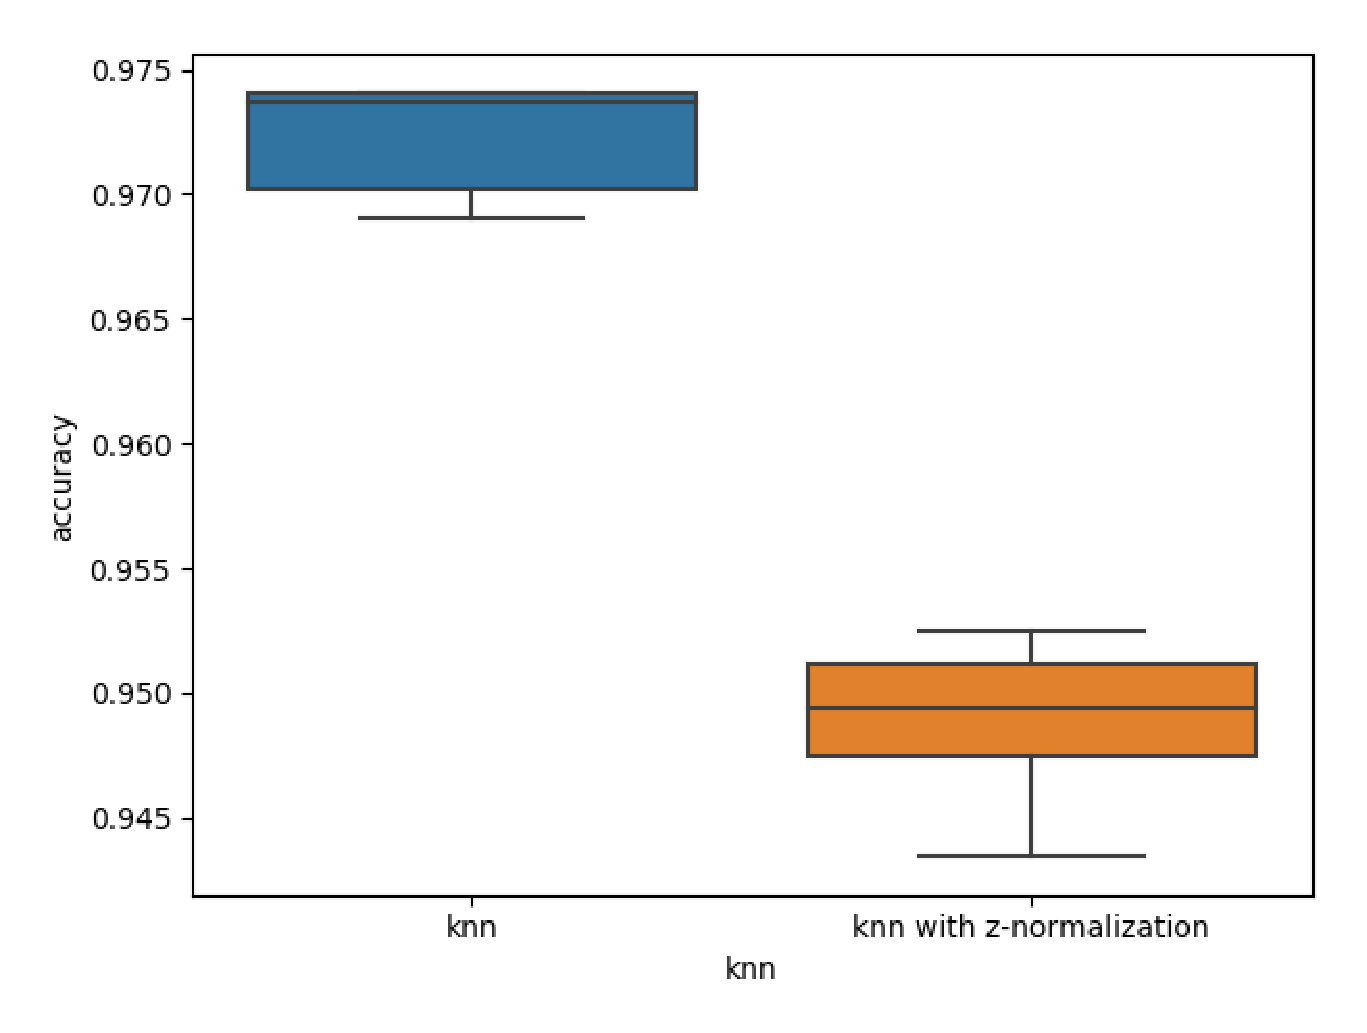
\includegraphics[width=0.5\linewidth]{figures/knn-z.eps}
    \caption{Affact of z-normalization }
    \label{fig:knnz}
  \end{figure}
  \end{itemize}
\end{slide}

\begin{slide}{Dimension Reduce}
  \begin{itemize}
    \item PCA
    \begin{itemize}
      \item is a statistical procedure that uses an orthogonal transformation to
      convert a set of observations of possibly correlated variables (entities 
      each of which takes on various numerical values) into a set of values of
      linearly uncorrelated variables called principal components -- WIKI \pause
    \end{itemize}
  \end{itemize}
  \begin{figure}[h]
    \centering
    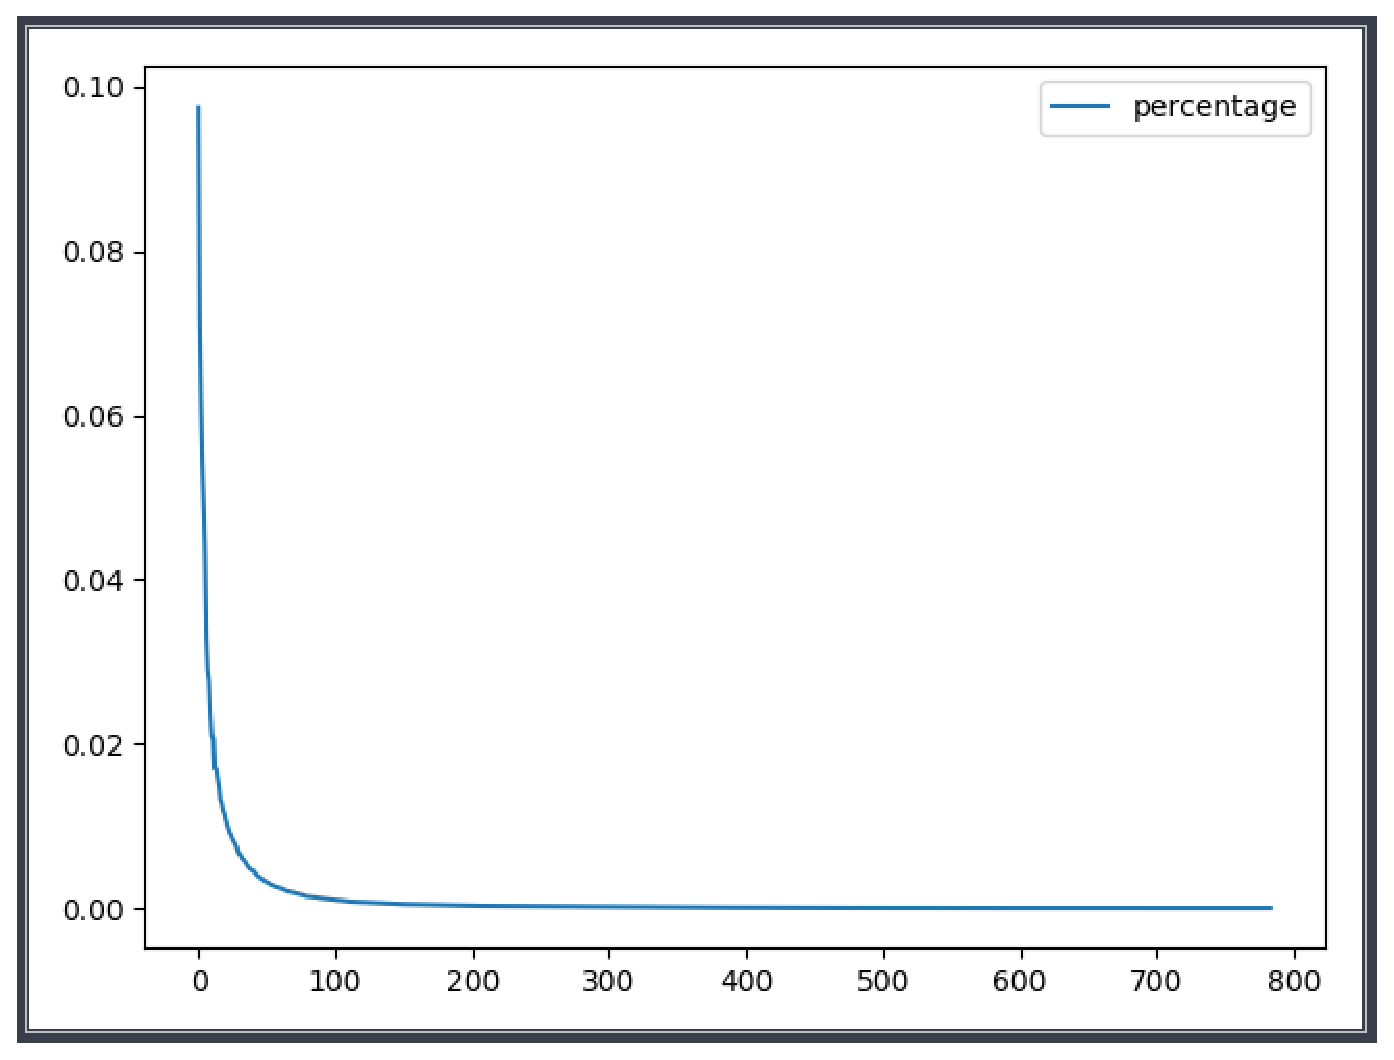
\includegraphics[width=0.5\linewidth]{figures/pca.eps}
    \caption{pca}
    \label{fig:pca}
  \end{figure}
\end{slide}

\begin{slide}{Dimension Reduce}
  \begin{itemize}
    \item PCA
    \begin{itemize}
      \item is a statistical procedure that uses an orthogonal transformation to
      convert a set of observations of possibly correlated variables (entities 
      each of which takes on various numerical values) into a set of values of
      linearly uncorrelated variables called principal components -- WIKI
    \end{itemize}
  \end{itemize}
  \begin{figure}[h]
    \centering
    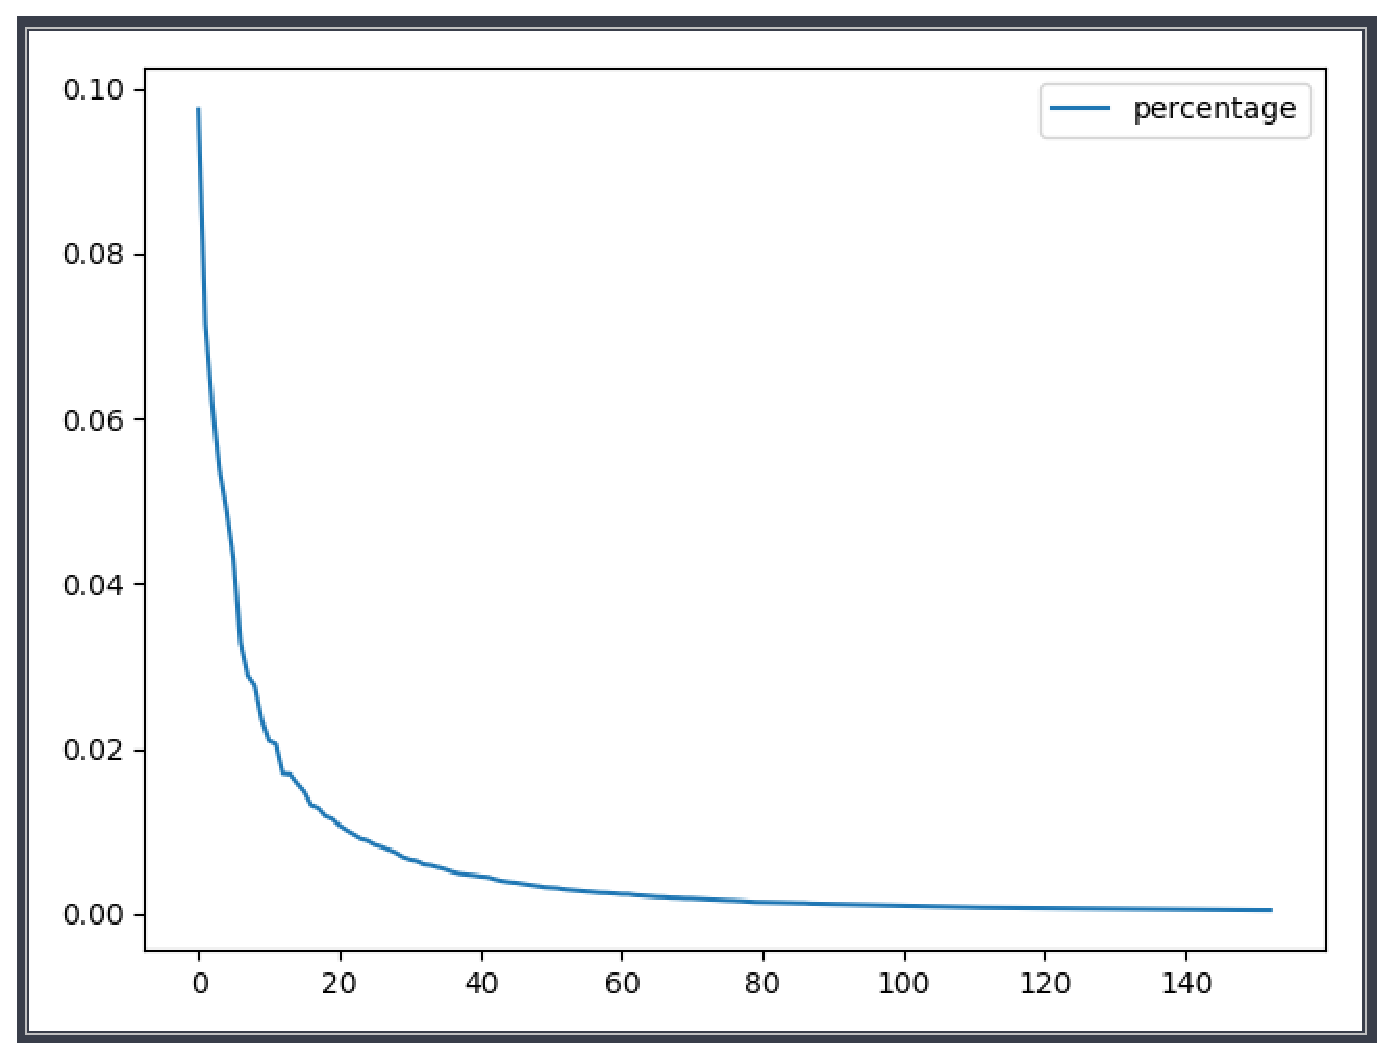
\includegraphics[width=0.5\linewidth]{figures/pca-140.eps}
    \caption{pca with 140 dimension}
    \label{fig:pca140}
  \end{figure}
\end{slide}

\begin{slide}{Dimension Reduce}
  \begin{itemize}
    \item PCA
    \begin{itemize}
      \item is a statistical procedure that uses an orthogonal transformation to
      convert a set of observations of possibly correlated variables (entities 
      each of which takes on various numerical values) into a set of values of
      linearly uncorrelated variables called principal components -- WIKI
    \end{itemize}
  \end{itemize}
  \begin{figure}[h]
    \centering
    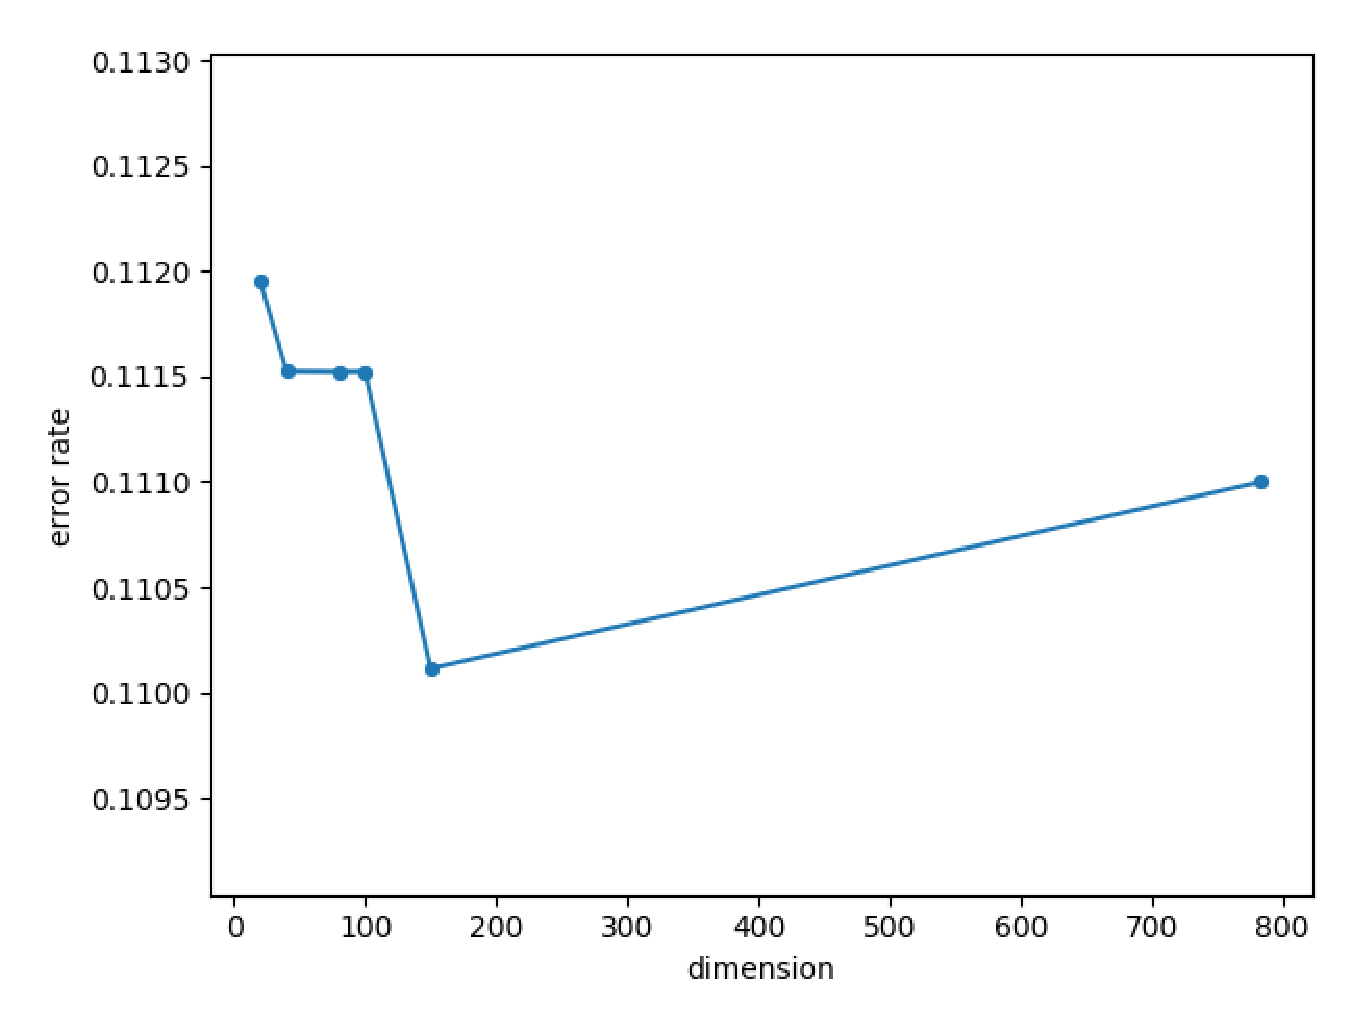
\includegraphics[width=0.5\linewidth]{figures/pca-de.eps}
    \caption{pca error rate on dimensions}
    \label{fig:pcade}
  \end{figure}
\end{slide}

\begin{slide}{Dimension Reduce}
  \begin{itemize}
    \item Let n_component of PCA be 40
  \end{itemize}
\end{slide}


\section{Model Selection}

\begin{slide}{K-means}
  \begin{itemize}
    \item Let n_clusters be 10 \pause
    \item Init centers randomly \pause
    \begin{figure}[h]
      \begin{minipage}[t]{0.4\linewidth}
        \centering
        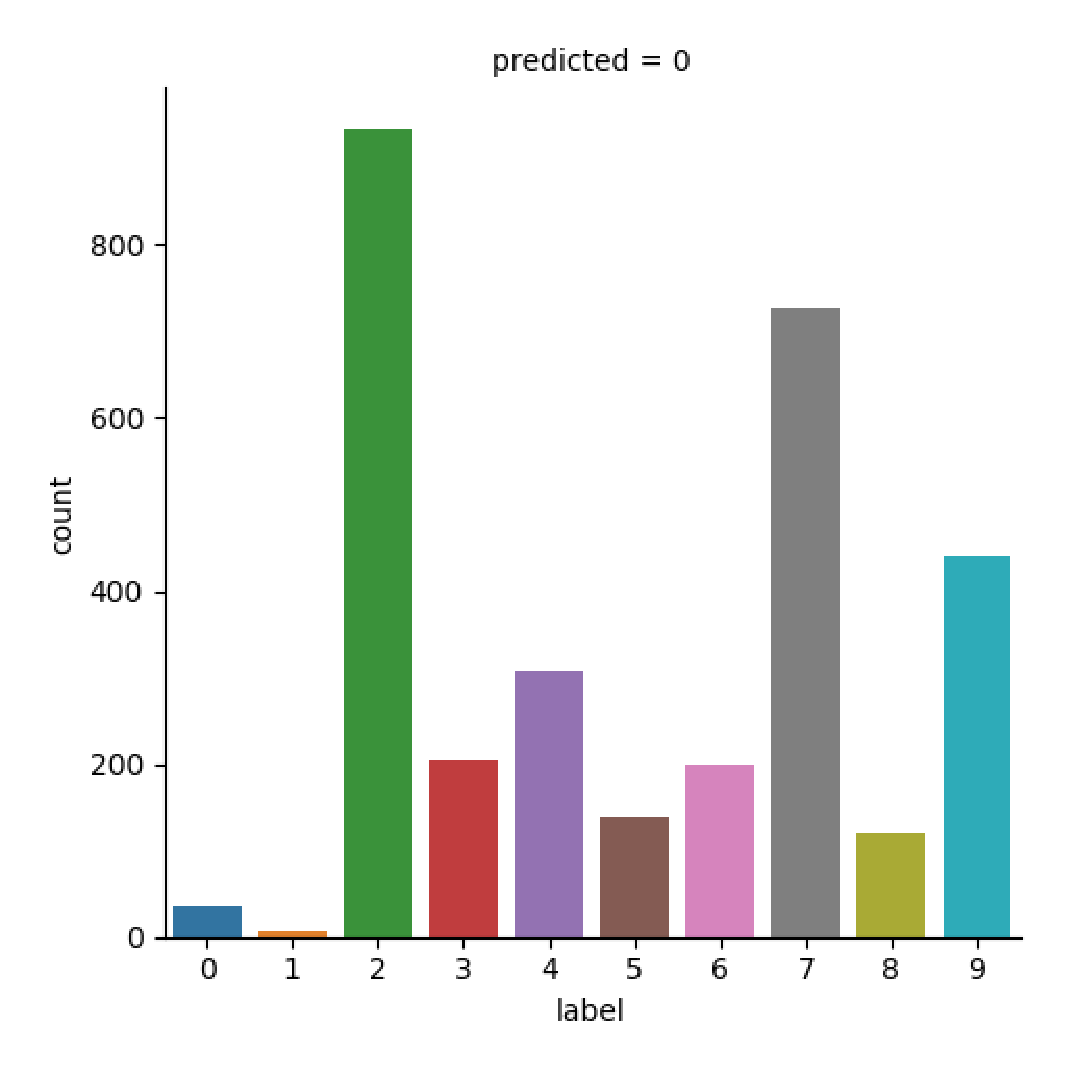
\includegraphics[width=1.2\textwidth]{figures/label-count0.eps}
        \caption{distribution of labels for 0}
        \label{fig:label-count0}
      \end{minipage}
      \pause
      \hfill
      \begin{minipage}[t]{0.4\linewidth}
        \centering
        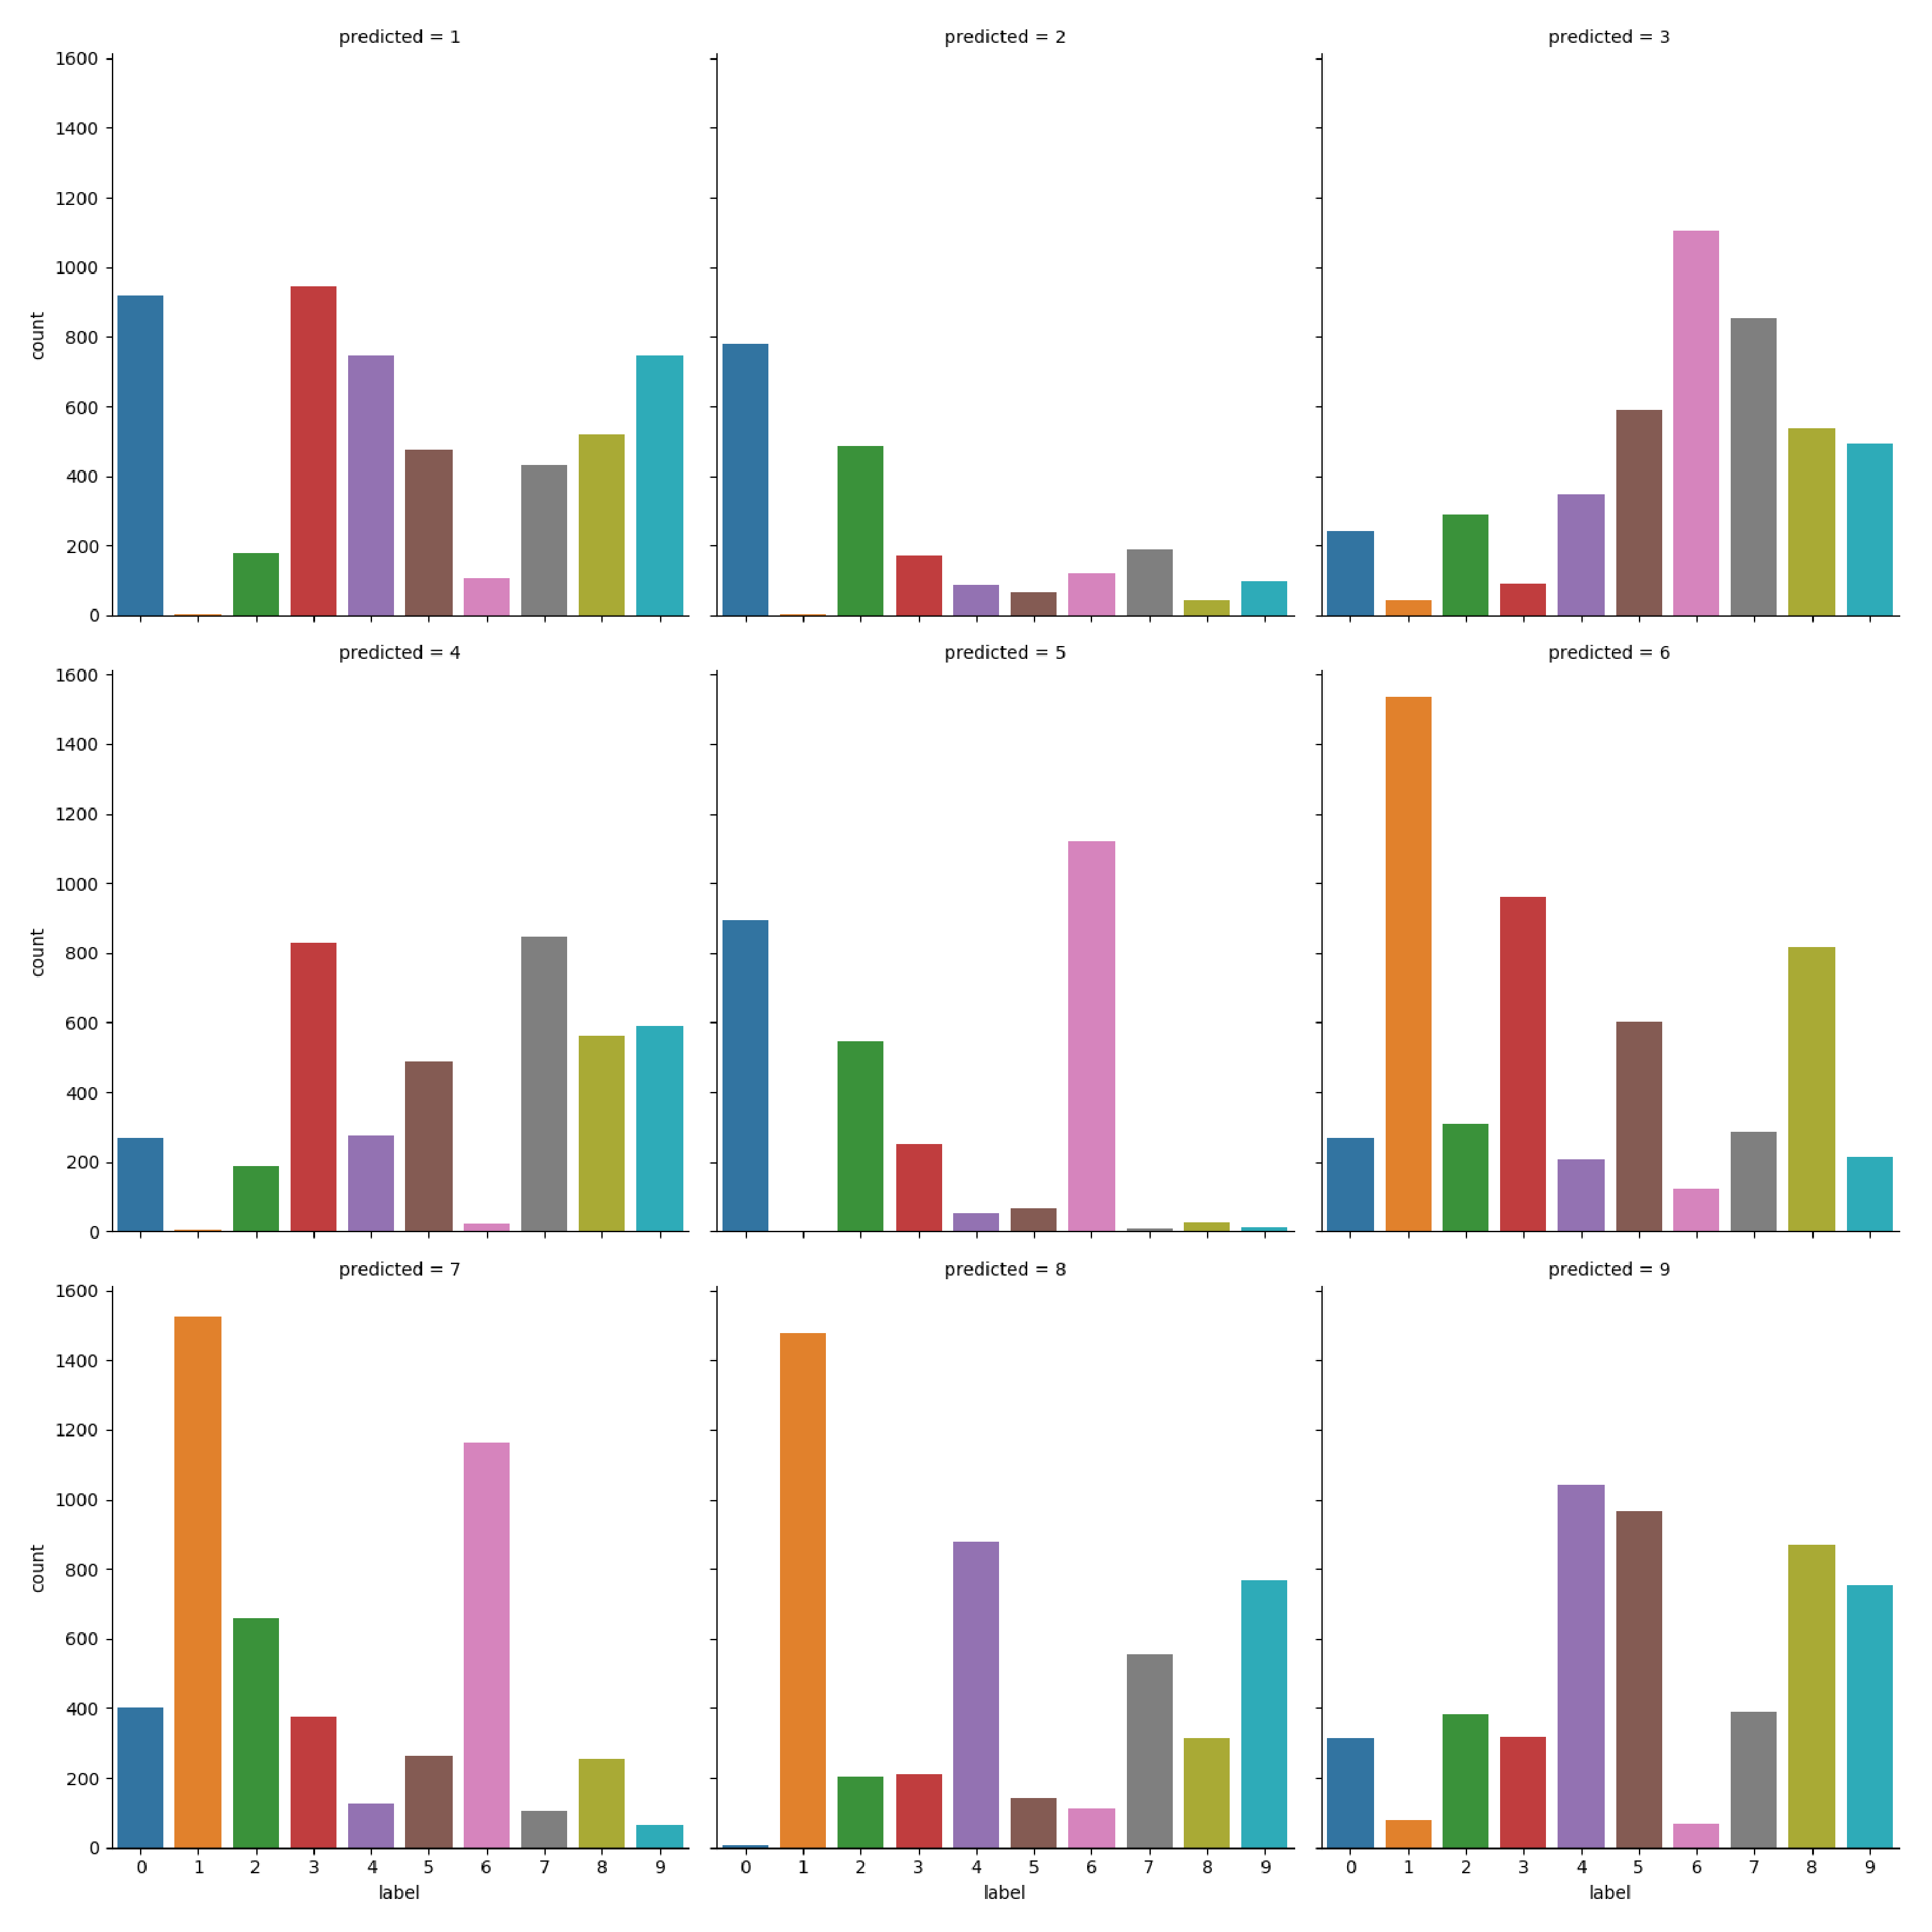
\includegraphics[width=1.2\textwidth]{figures/label-count-9.eps}
        \caption{distribution of labels}
        \label{fig:label-count-9}
      \end{minipage} 
    \end{figure}
  \end{itemize}
\end{slide}

\begin{slide}{SVM}
  \begin{itemize}
  \item GridSearchCV \pause
  \item parameters = {'kernel': ('linear', 'poly', 'rbf')} \pause
  \item mean of scores under 5-fold cv: 0.891405
  \end{itemize}
\end{slide}

\begin{slide}{KNN}
  \begin{itemize}
    \item is a non-parametric method used for classification and regression.
    In both cases, the input consists of the k closest training examples in
    the feature space \pause
    \item selection of K
  \end{itemize}
  \begin{figure}[h]
    \centering
    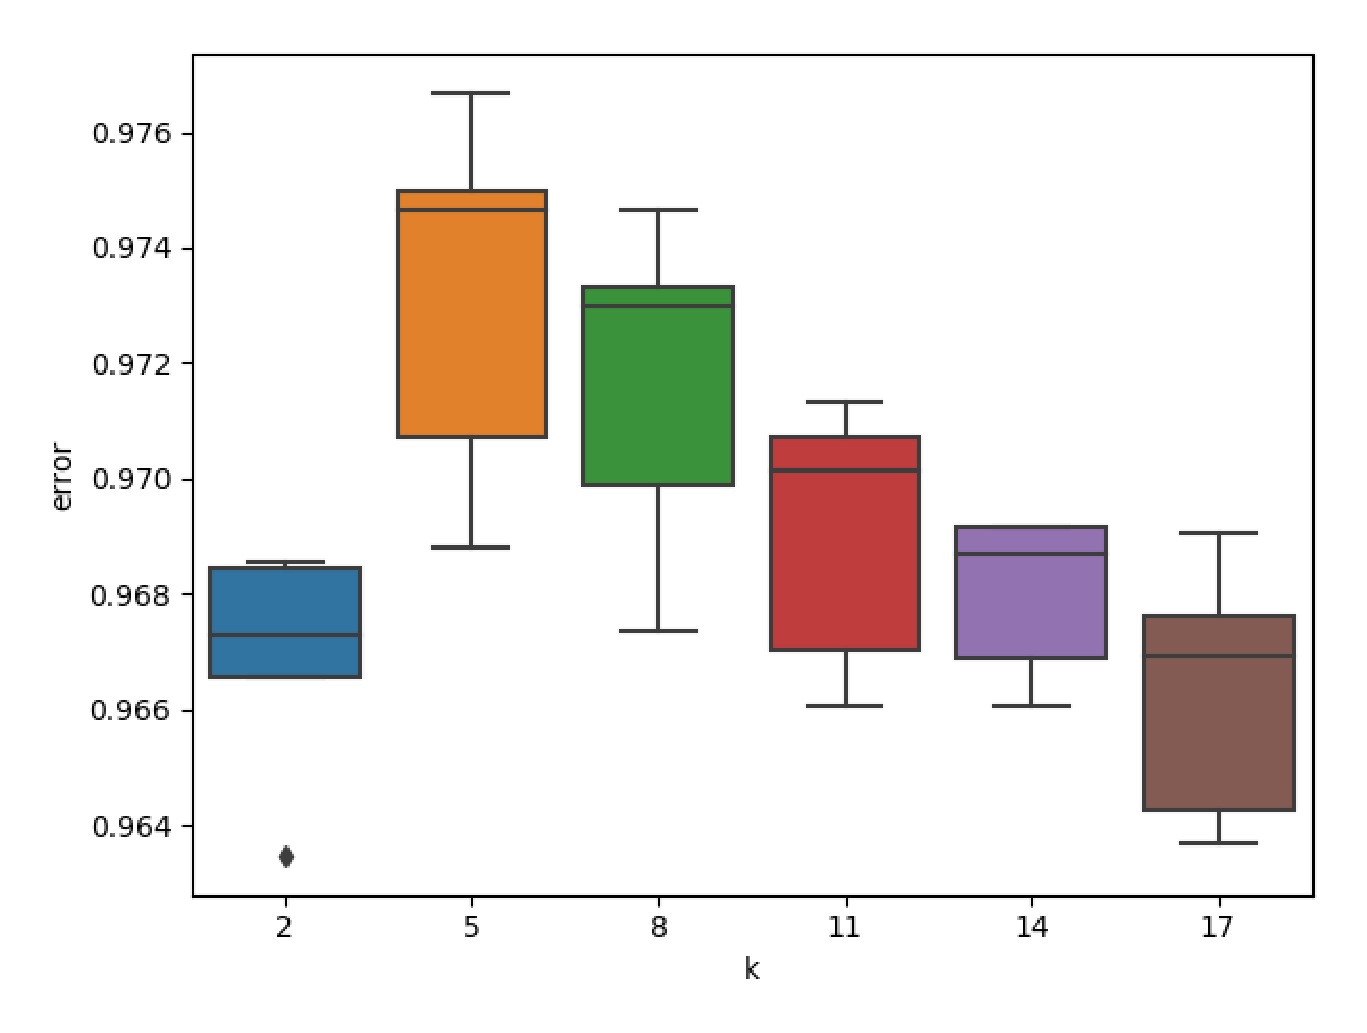
\includegraphics[width=0.5\linewidth]{figures/knn-k.eps}
    \caption{accurary of knn with different Ks}
    \label{fig:knn-k}
  \end{figure}
\end{slide}

\begin{slide}{CNN-Constructure}
  \begin{itemize}
    \item one layer \pause
    \begin{figure}[h]
      \centering
      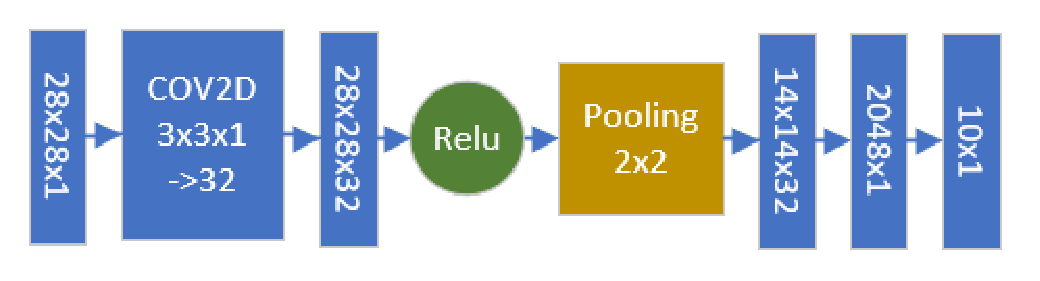
\includegraphics[width=0.5\linewidth]{figures/layer1.eps}
      \caption{One Layer}
      \label{fig:one-layer}
    \end{figure}
    \pause
    \item Three layer \pause
    \begin{figure}[h]
      \centering
      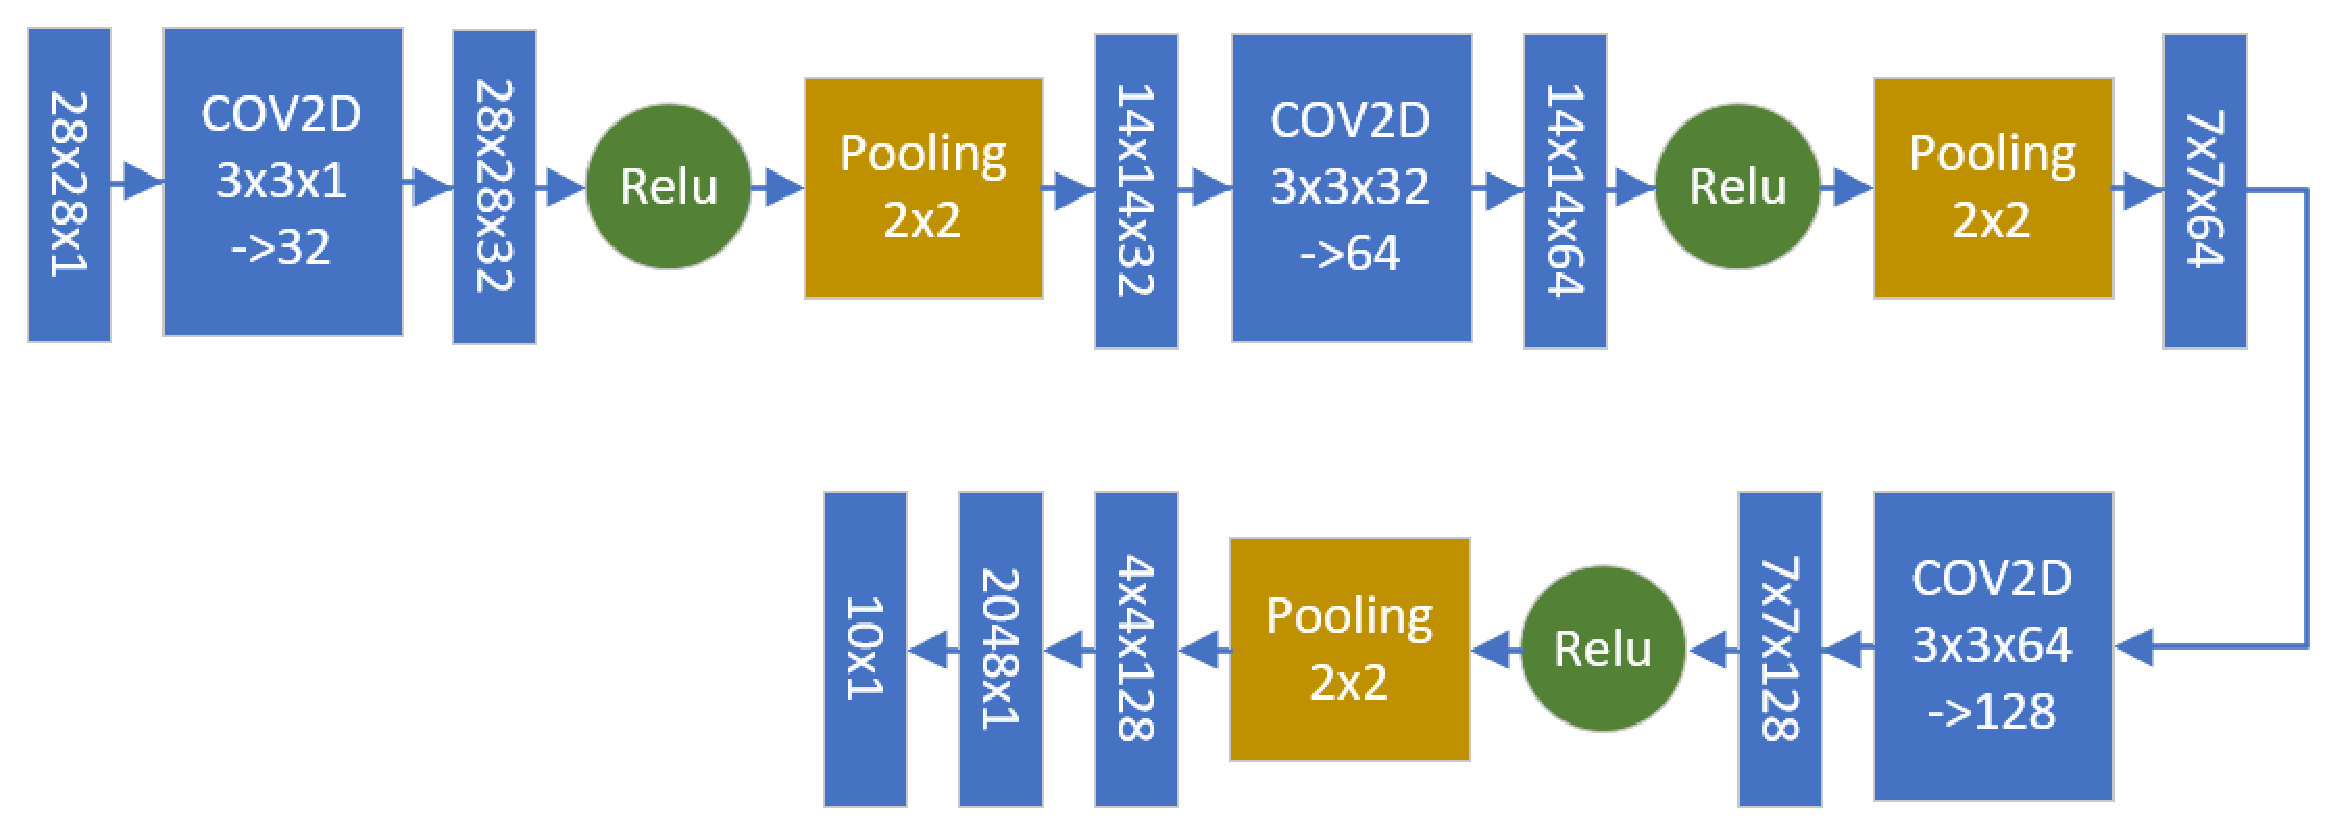
\includegraphics[width=0.7\textwidth]{figures/layer3.eps}
      \caption{Three Layer}
      \label{fig:three-layer}
    \end{figure}  
  \end{itemize}
\end{slide}

\begin{slide}{CNN-Tune and Validate}
  \begin{itemize}
    \item Loss function: softmax_cross_entropy_with_logits
    \item Optimizer: RMSPropOptimizer
    \item Comparation of 5-fold CV between two mode
  \end{itemize}
  \begin{figure}[h]
    \centering
    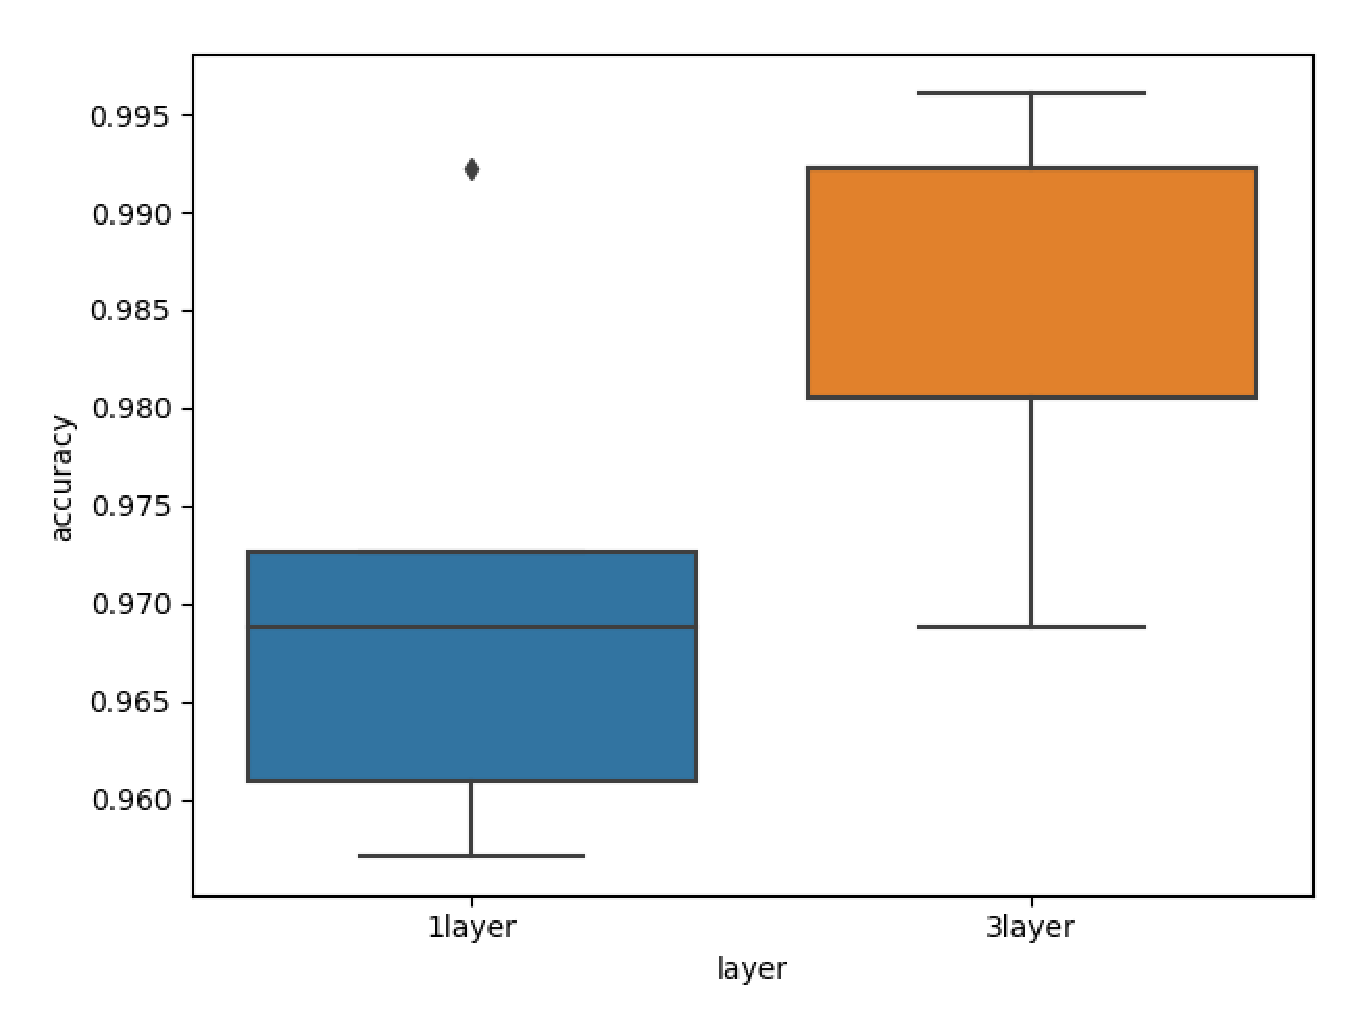
\includegraphics[width=0.5\textwidth]{figures/compare-layers.eps}
    \caption{Comparation between two models}
    \label{fig:comparation-two-models}
  \end{figure}  
\end{slide}

\begin{slide}{Comparation among Different Models}
  \begin{figure}[h]
    \centering
    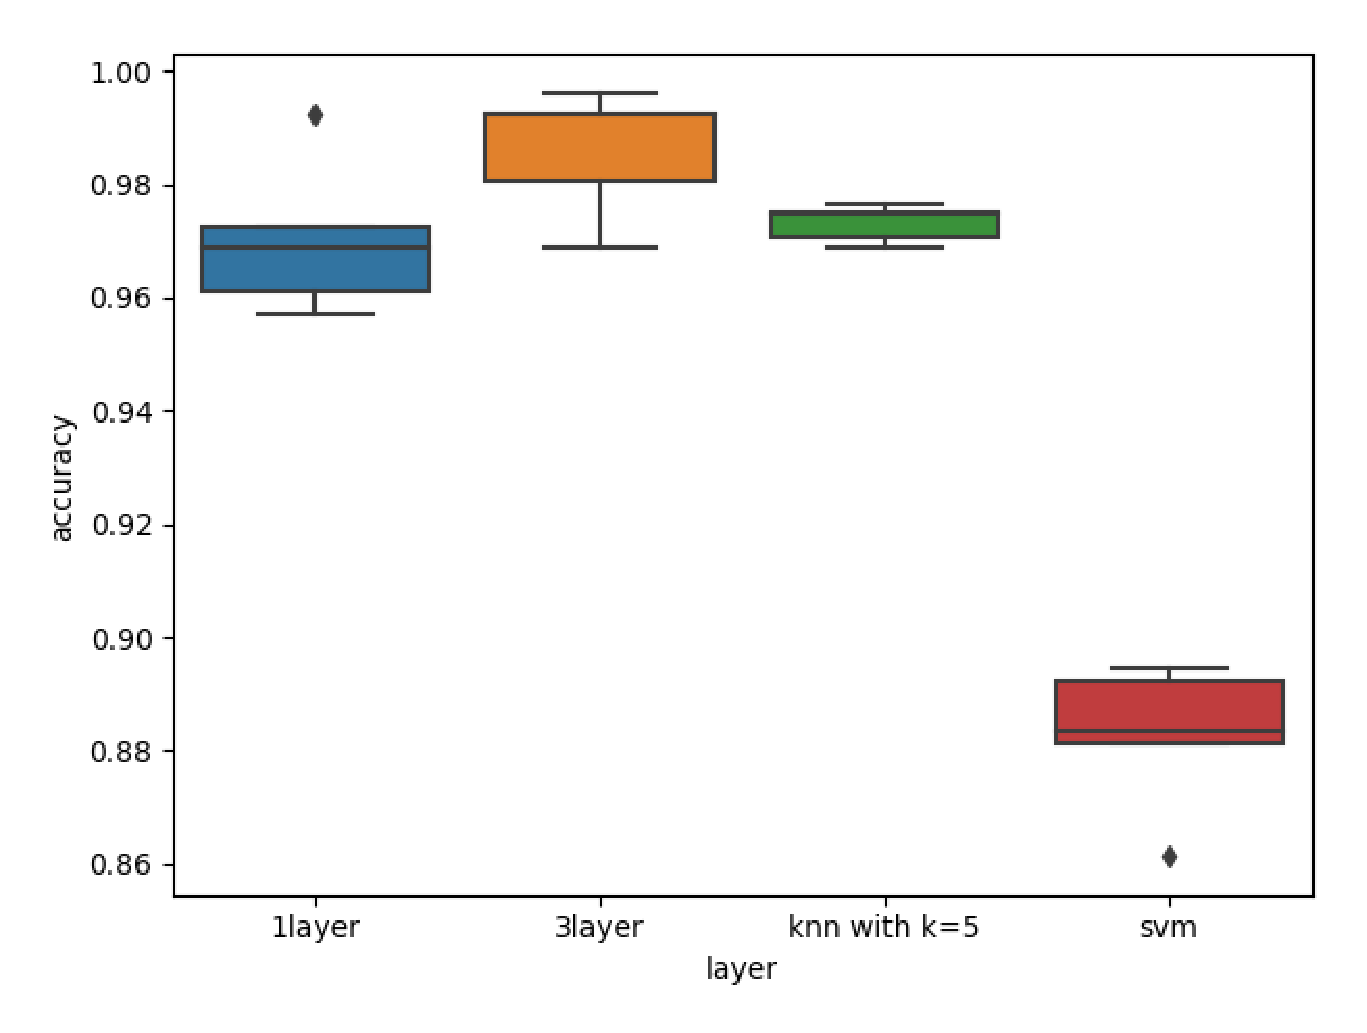
\includegraphics[width=0.5\textwidth]{figures/comparation.eps}
    \caption{Comparation}
    \label{fig:comparation}
  \end{figure}  
\end{slide}

\section{Experiment}

\begin{slide}{Rank of Competition}
  \begin{itemize}
    \item Score: 0.98957
    \item Rank: 1233/2723
  \end{itemize}
  \begin{figure}[h]
    \centering
    
\includegraphics[width=0.8\textwidth]{figures/competition.eps}
    \caption{Result of the best submission}
    \label{fig:result-of-best-submission}
  \end{figure} 
\end{slide}


\section{Summary}

\begin{slide}{Thanks}
  \begin{itemize}
    \item Thanks for listening~
  \end{itemize}
\end{slide}

% \begin{slide}{References (1)}
% \bibliographystyle{plain}
% \nobibliography{YourBib}
% \bibentry{someone1}
% \bibentry{someone2}
% \end{slide}
% \begin{slide}{References (2)}
% \bibentry{someone3}
% \end{slide}

% \begin{slide}{Slide}
% \cite{someone}
% \end{slide}
% 
% \begin{slide}{References}
% \bibliographystyle{plain}
% % \bibliography{YourBib}
% \end{slide}

\end{document}

\endinput
